% This file was created with matplot2tikz v0.5.4.
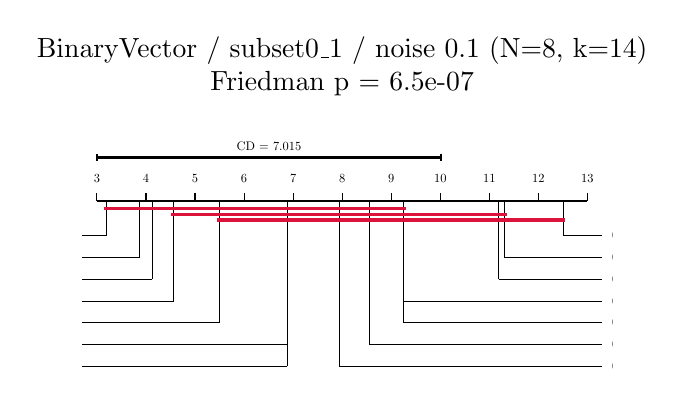
\begin{tikzpicture}

\definecolor{crimson}{RGB}{220,20,60}
\definecolor{darkgray176}{RGB}{176,176,176}

\begin{axis}[
hide x axis,
hide y axis,
tick align=outside,
tick pos=left,
title style={align=center},
title={BinaryVector / subset0\_1 / noise 0.1  (N=8, k=14)\\Friedman p = 6.5e-07},
x grid style={darkgray176},
xmin=2.5, xmax=13.5,
xtick style={color=black},
y grid style={darkgray176},
ymin=-8.5, ymax=1.8,
ytick style={color=black}
]
\addplot [black]
table {%
3 0
13 0
};
\addplot [black]
table {%
3 0
3 0.18
};
\addplot [black]
table {%
4 0
4 0.18
};
\addplot [black]
table {%
5 0
5 0.18
};
\addplot [black]
table {%
6 0
6 0.18
};
\addplot [black]
table {%
7 0
7 0.18
};
\addplot [black]
table {%
8 0
8 0.18
};
\addplot [black]
table {%
9 0
9 0.18
};
\addplot [black]
table {%
10 0
10 0.18
};
\addplot [black]
table {%
11 0
11 0.18
};
\addplot [black]
table {%
12 0
12 0.18
};
\addplot [black]
table {%
13 0
13 0.18
};
\addplot [line width=0.32pt, black]
table {%
3.1875 0
3.1875 -0.8
};
\addplot [line width=0.32pt, black]
table {%
3.1875 -0.8
2.7 -0.8
};
\addplot [line width=0.32pt, black]
table {%
3.875 0
3.875 -1.3
};
\addplot [line width=0.32pt, black]
table {%
3.875 -1.3
2.7 -1.3
};
\addplot [line width=0.32pt, black]
table {%
4.125 0
4.125 -1.8
};
\addplot [line width=0.32pt, black]
table {%
4.125 -1.8
2.7 -1.8
};
\addplot [line width=0.32pt, black]
table {%
4.5625 0
4.5625 -2.3
};
\addplot [line width=0.32pt, black]
table {%
4.5625 -2.3
2.7 -2.3
};
\addplot [line width=0.32pt, black]
table {%
5.5 0
5.5 -2.8
};
\addplot [line width=0.32pt, black]
table {%
5.5 -2.8
2.7 -2.8
};
\addplot [line width=0.32pt, black]
table {%
6.875 0
6.875 -3.3
};
\addplot [line width=0.32pt, black]
table {%
6.875 -3.3
2.7 -3.3
};
\addplot [line width=0.32pt, black]
table {%
6.875 0
6.875 -3.8
};
\addplot [line width=0.32pt, black]
table {%
6.875 -3.8
2.7 -3.8
};
\addplot [line width=0.32pt, black]
table {%
7.9375 0
7.9375 -3.8
};
\addplot [line width=0.32pt, black]
table {%
7.9375 -3.8
13.3 -3.8
};
\addplot [line width=0.32pt, black]
table {%
8.5625 0
8.5625 -3.3
};
\addplot [line width=0.32pt, black]
table {%
8.5625 -3.3
13.3 -3.3
};
\addplot [line width=0.32pt, black]
table {%
9.25 0
9.25 -2.8
};
\addplot [line width=0.32pt, black]
table {%
9.25 -2.8
13.3 -2.8
};
\addplot [line width=0.32pt, black]
table {%
9.25 0
9.25 -2.3
};
\addplot [line width=0.32pt, black]
table {%
9.25 -2.3
13.3 -2.3
};
\addplot [line width=0.32pt, black]
table {%
11.1875 0
11.1875 -1.8
};
\addplot [line width=0.32pt, black]
table {%
11.1875 -1.8
13.3 -1.8
};
\addplot [line width=0.32pt, black]
table {%
11.3125 0
11.3125 -1.3
};
\addplot [line width=0.32pt, black]
table {%
11.3125 -1.3
13.3 -1.3
};
\addplot [line width=0.32pt, black]
table {%
12.5 0
12.5 -0.8
};
\addplot [line width=0.32pt, black]
table {%
12.5 -0.8
13.3 -0.8
};
\addplot [thick, black]
table {%
3 1
10.0145947931247 1
};
\addplot [thick, black]
table {%
3 0.92
3 1.08
};
\addplot [thick, black]
table {%
10.0145947931247 0.92
10.0145947931247 1.08
};
\addplot [very thick, crimson]
table {%
3.1375 -0.18
9.3 -0.18
};
\addplot [very thick, crimson]
table {%
4.5125 -0.31
11.3625 -0.31
};
\addplot [very thick, crimson]
table {%
5.45 -0.44
12.55 -0.44
};
\draw (axis cs:3,0.32) node[
  scale=0.45,
  anchor=south,
  text=black,
  rotate=0.0
]{3};
\draw (axis cs:4,0.32) node[
  scale=0.45,
  anchor=south,
  text=black,
  rotate=0.0
]{4};
\draw (axis cs:5,0.32) node[
  scale=0.45,
  anchor=south,
  text=black,
  rotate=0.0
]{5};
\draw (axis cs:6,0.32) node[
  scale=0.45,
  anchor=south,
  text=black,
  rotate=0.0
]{6};
\draw (axis cs:7,0.32) node[
  scale=0.45,
  anchor=south,
  text=black,
  rotate=0.0
]{7};
\draw (axis cs:8,0.32) node[
  scale=0.45,
  anchor=south,
  text=black,
  rotate=0.0
]{8};
\draw (axis cs:9,0.32) node[
  scale=0.45,
  anchor=south,
  text=black,
  rotate=0.0
]{9};
\draw (axis cs:10,0.32) node[
  scale=0.45,
  anchor=south,
  text=black,
  rotate=0.0
]{10};
\draw (axis cs:11,0.32) node[
  scale=0.45,
  anchor=south,
  text=black,
  rotate=0.0
]{11};
\draw (axis cs:12,0.32) node[
  scale=0.45,
  anchor=south,
  text=black,
  rotate=0.0
]{12};
\draw (axis cs:13,0.32) node[
  scale=0.45,
  anchor=south,
  text=black,
  rotate=0.0
]{13};
\draw (axis cs:2.6,-0.8) node[
  scale=0.45,
  anchor=east,
  text=black,
  rotate=0.0
]{ECC  (3.19)};
\draw (axis cs:2.6,-1.3) node[
  scale=0.45,
  anchor=east,
  text=black,
  rotate=0.0
]{LP  (3.88)};
\draw (axis cs:2.6,-1.8) node[
  scale=0.45,
  anchor=east,
  text=black,
  rotate=0.0
]{CC  (4.12)};
\draw (axis cs:2.6,-2.3) node[
  scale=0.45,
  anchor=east,
  text=black,
  rotate=0.0
]{BR  (4.56)};
\draw (axis cs:2.6,-2.8) node[
  scale=0.45,
  anchor=east,
  text=black,
  rotate=0.0
]{MLkNN  (5.50)};
\draw (axis cs:2.6,-3.3) node[
  scale=0.45,
  anchor=east,
  text=black,
  rotate=0.0
]{IA4  (6.88)};
\draw (axis cs:2.6,-3.8) node[
  scale=0.45,
  anchor=east,
  text=black,
  rotate=0.0
]{IA2  (6.88)};
\draw (axis cs:13.4,-3.8) node[
  scale=0.45,
  anchor=west,
  text=black,
  rotate=0.0
]{(7.94)  IA1};
\draw (axis cs:13.4,-3.3) node[
  scale=0.45,
  anchor=west,
  text=black,
  rotate=0.0
]{(8.56)  IA3};
\draw (axis cs:13.4,-2.8) node[
  scale=0.45,
  anchor=west,
  text=black,
  rotate=0.0
]{(9.25)  IA8};
\draw (axis cs:13.4,-2.3) node[
  scale=0.45,
  anchor=west,
  text=black,
  rotate=0.0
]{(9.25)  IA6};
\draw (axis cs:13.4,-1.8) node[
  scale=0.45,
  anchor=west,
  text=black,
  rotate=0.0
]{(11.19)  IA7};
\draw (axis cs:13.4,-1.3) node[
  scale=0.45,
  anchor=west,
  text=black,
  rotate=0.0
]{(11.31)  IA5};
\draw (axis cs:13.4,-0.8) node[
  scale=0.45,
  anchor=west,
  text=black,
  rotate=0.0
]{(12.50)  CLR};
\draw (axis cs:6.50729739656237,1.15) node[
  scale=0.45,
  anchor=base,
  text=black,
  rotate=0.0
]{CD = 7.015};
\end{axis}

\end{tikzpicture}
